\documentclass[11pt]{amsart}
%\usepackage{geometry}                % See geometry.pdf to learn the layout options. There are lots.
%\geometry{letterpaper}                   % ... or a4paper or a5paper or ... 
%\geometry{landscape}                % Activate for for rotated page geometry
%\usepackage[parfill]{parskip}    % Activate to begin paragraphs with an empty line rather than an indent
\usepackage{graphicx}
\usepackage{amssymb}
\usepackage{epstopdf}
%\usepackage{todonotes}
\usepackage[dvipsnames]{xcolor}
\usepackage{tikz}
\usepackage{bayesnet}

\newcommand{\ndg}[1]{{\color{ForestGreen}[#1]}}


\DeclareGraphicsRule{.tif}{png}{.png}{`convert #1 `dirname #1`/`basename #1 .tif`.png}


\usepackage{stmaryrd}
\newcommand{\denote}[1]{\llbracket#1\rrbracket}
%\left\llbracket\;\text{#2}\;\right\rrbracket^{#1}


\title{A quantitative study of vague language}
\author{Noah D.~Goodman}
%\date{}                                           % Activate to display a given date or no date

\begin{document}
\maketitle

\section{Introduction}

When does a movie stop being \emph{good}?
Is a five-foot man \emph{short}? 
And, how many hairs can you have and still be \emph{bald}?
These are all questions that seem not to have an answer, because the language used is \emph{vague}.
Vagueness is extremely common in everyday language, being perhaps the rule rather than exceptional.
This has important implications. 
For instance, the legal doctrine of \ndg{whatsit} allows local statutes to be invalidated if they are determined to be vague \ndg{true?}.
\ndg{something about AI / internet / NLP?}
%
Vagueness may also expose for study critical features of the psychological structure of language and cognition.
The lack of clear truth-conditions has been the most persistent obstacle to the use of mathematical logic as a model of human thought (which is indeed what mathematical logic was initially developed for \cite{bool}).
The silver lining for experimental psychology is that vagueness implies quantitative, graded data where otherwise there might only be binary truth values; there is more information in a number than a bit. 
Indeed, it was precisely the vague boundaries of everyday concepts that drove psychological research to develop the notions of prototype and typicality \cite{rosch}.
While this line of research yielded successful quantitative models of category generalization \cite{GCM,RR, ..}, less progress has been made at connecting theories of vague language to psychological data.
In this paper we describe and evaluate a quantitative theory of vague adjectives. 

Vague concepts are characterized by having borderline cases: instances that are neither clearly in nor clearly out, even if one knows everything about that instance. 
For instance, having measured a man's height down to a millimeter, it may still be impossible to determine if that man is \emph{tall}.
The puzzle of vagueness goes back thousands of years, at least to the ancient greek philosopher \ndg{whatshisface}, who created a series of logic puzzles that hinged on vague language. 
The most famous is known as the \emph{sorites}, or paradox of the heap:
\begin{enumerate}
\item A million grains of sand together are a heap.
\item If you take one grain of sand from a heap, it is still a heap.
\item One grain of sand is a heap.
\end{enumerate}
People tend to happily endorse the first two sentences, but resoundingly reject the last sentence. Yet by mathematical induction the last statement should follow from the first two.
While this puzzle has often been taken as a problem for logic or metaphysics, we instead view it as a psychological issue. What could be the process of interpretation and endorsement that would lead to the observed pattern of agreement?

\ndg{should mention sorites series form?}

As formulated above the sorites involves vague nouns, such as \emph{heap}. 
Many features of noun concepts make it hard to isolate the origin of their vagueness; they are high-dimensional and likely depend on function and relation \cite{stuff}.
Adjectives, on the other hand, demonstrate the key properties of vagueness---borderline cases and the sorites---but usually depend on a single critical scale.
For instance, \emph{tall} seems to depend on height alone, and \emph{expensive} on price.
This make adjectival vagueness a more tractable ground for model building---at least that is our motivation for considering adjective in this paper.
Vagueness is characterized by borderline cases and the sorites.
Bordeline cases, and gradedness, are clearly possible for adjectives; it is not hard to create sorites arguments for adjectives paralleling the one above:
\begin{enumerate}
\item A million-dollar watch is expensive.
\item A watch that costs one dollar less than an expensive watch is still expensive.
\item A one-dollar watch is expensive.
\end{enumerate}
In the remainder we refer to sentences like (1) as our \emph{concrete} sentences and sentences like (2) as \emph{inductive}.
Vague adjectives have a third key property, related to the others: they are relative, depending critically on the class. 
For instance an \emph{expensive watch} is likely very different in price from an \emph{expensive house}.
Thus the challenge is to experimentally establish that these three properties and explain their quantitative pattern with a formal model of interpretation. \ndg{revise that last sentence.}

It is remarkably easy for people to evaluate sentences like 1--3, forming an opinion about their truthiness consistently and without much reflection. This and the prevalence of vague utterances both suggest that vagueness is central to the design of language---a feature not a bug. We will suggest that vagueness indeed follows from basic aspects of the architecture of language: underspecified literal meanings coupled with pragmatic inference that fills in meaning by reasoning about the speaker's intent, in a conversational context.
\ndg{more on uRSA}

\ndg{related research??}
\cite{Dzhafarov2014}
%%From dan:
%%Only thing I know of that's at all directly relevant:
%%http://www.psych.purdue.edu/~ehtibar/publications/DzhPerry.APP.rev.pdf
%%that's experimental but not about our kind of sorites. the link is spelled out a bit more, in theoretical terms, in a couple of nice papers by Paul Egre, eg here:
%%http://link.springer.com/chapter/10.1007%2F978-3-642-18446-8_5
%%Of course there's a bunch of other stuff related to vagueness, e.g. on the acceptability of "f & not f" for borderline f, but nothing that deals with sorites per se. 

In the remainder of this paper we \ndg{first?} focus on the scale of price and the adjective \emph{expensive}. This is a useful case study because people have robust prior knowledge of prices for different common object types, and prices can be referred to directly (people can report and comprehend prices as numbers, unlike other scales, such as \emph{goodness}).
In section \ref{exp1} we collect data for endorsement of concrete and inductive sentences, and show that the three characteristics of vague adjectives are evident: gradedness (including borderline cases), dependence on category (relativity), and sometimes strong endorsement of inductive sentences.
We then introduce a model of adjectival vagueness in section \ref{model}, which realizes adjective meanings as underspecified degree comparisons and fixes meaning through a pragmatic inference. \ndg{uRSA}
This model depends on non-linguistic background knowledge; in section \ref{priors} we elicit the prior distribution on prices for several different categories of everyday item.
We find that the model predictions, given these elicited priors, provide a good match the human data from Experiment 1.
In section \ref{exp3} we replicate and extend this finding, using a wider range of prices in the target sentences.
\ndg{In section \ref{something} we consider other adjectival scales, showing something.}
We conclude by considering the implications of our results for language and cognition, and the relationship of our model to other theories of vagueness.



\section{Experiment 1}
\label{exp1}

\subsection{Participants}

$N=70$ participants for Experiment 1a and $N=50$ participants for Experiment 1b were recruited through Amazon's Mechanical turk.\footnote{The number of subjects was chosen based on... \ndg{what}?} 
Only participants with U.S.~IP addresses and approval rate above XX were recruited \ndg{check}.
Participants were paid for their time.

\subsection{Materials}

We generated a set of concrete sentences of the form ``A \{X\} that costs \$\{P\} is expensive.'' 
There were five target categories ``X'': headphones, laptop, watch, coffee maker, and sweater.
The target price ``P'' had XX different values for each category, chosen by the experimenters' intuition for a reasonable range of plausibility.

We also generated a set of inductive sentences. 
In Experiment 1a, they had the relative clause form ``A \{X\} that costs \$\{P\} less than an expensive \{X\} is also expensive.''
The inductive sentences for Experiment 1b instead had the conditional form ``If a \{X\} is expensive, then another \{X\} that costs \$\{P\} less is also expensive.''
In both cases, we used the same five target categories ``X''. 
There were XX target price gaps ``P'' per category, again chosen by intuition with the goal of yielding both good inductive premises and more questionable ones.

\subsection{Methods}

Participants completed 55 trials in about ten minutes.
Participants were instructed:

\begin{quote}
In this experiment, we would like you to give us your opinion about some statements. Each statement is about the prices of different household items.

For each question, please indicate how much you agree with the statement. Choose a circle that is closer to the words "Completely agree" if you agree and choose a circle that is closer to the words "Completely disagree" if you disagree.
\end{quote}

Each participant was then asked to rate a series of sentences on a nine-point scale.
\ndg{WHAT WAS THE DESIGN?}
Each participant then saw all five categories with all four price values for each kind of sentence \ndg{yielding 5 x 5 x 2 = 50???}; trials were presented in random order.

%We ran two different versions of the sorites experiment, with two different phrasings. In both versions, participants saw two different kinds of questions regarding 5 different categories of objects. These questions were all randomly intermixed. One of the kinds of questions represented the concrete premise and one represented the inductive premise. Participants were asked to rate each of these questions on a 9-point Likert scale from ?Completely disagree? (1) to ?Completely agree? (9).
%The two versions of the experiment differed in their phrasing of the inductive premise. Version 1 (N=70) used the relative clause phrasing ?An X that costs $? less than an expensive X is also expensive?. Version 2 (N=50) used the conditional statement phrasing ?If an X is expensive, then an X that costs $? less is also expensive?. 


\subsection{Results}


Judgements for inductive sentences of Experiment 1a and 1b had an extremely strong correlation of $r=0.98$. \ndg{double shcek that this is correlation of just inductive sentences.} We therefore combine data from the two experiments for the remainder of the analyses.

it is reliable (people agree: split half? beta?).
we qualitatively capture the three characteristic effects of vagueness:
  we see that judgements depend on the class (and on the price and frame).
  we see gradedness in endorsement of concrete premises, including borderline cases.
  we see strong endorsement of some inductive premises. importantly this is also graded, with some inductive sentences judged as not good at all.
  
this suggests rich quantitative patterns to explain.


\section{Model}
\label{model}

we make an uRSA model building on (or just using?) \cite{lassiter2015}.

\begin{figure}
\tikz{
  \node[latent,] (mu) {$\mu_i$};
  \node[latent, right=of mu] (sig) {$\sigma_i$};
  
  \node[above=of mu] (mumax) {$\mu^{max}$};
  \node[above=of sig] (sigmax) {$\sigma^{max}$};
  
  \node[latent, right=of sigmax] (sigbin) {$\sigma_{bin}$};

  \node[det, below=of mu, below=of sig] (pbin) {$P_{ib}$};
  \node[obs, below=of pbin] (dbin) {$d_{ib}$};
  
  \node[latent, right=of sigbin] (alpha) {$\alpha$};
  \node[above=of alpha] (alphamax) {$\alpha^{max}$};
  \node[right=of alphamax] (costmax) {$c_{max}$};
  \node[latent, below=of costmax] (cost) {$c$};

  \node[latent, below=of pbin, xshift=2cm] (s2concrete) {$S(C_{iv})$};
  \node[latent, right=of s2concrete, xshift=.25cm] (s2inductive) {$S(I_{i\varepsilon})$};
  
  \node[obs, below=of s2inductive] (sI) {$s^{I}_{i\varepsilon}$};
  \node[obs, below=of s2concrete] (sC) {$s^{C}_{iv}$};
  
  \node[above=of sigbin] (sigbinmax) {$\sigma_{bin}^{max}$};
  
  \edge {mumax} {mu}
  \edge {sigmax} {sig}
  \edge {mu, sig} {pbin}
  \edge {pbin, sigbin} {dbin}
  \edge {pbin} {s2inductive, s2concrete}
  \edge {s2inductive} {sI}
  \edge {s2concrete} {sC}
  \edge {alpha} {s2concrete, s2inductive}
  \edge {alphamax} {alpha}
  \edge {cost} {s2concrete, s2inductive}
  \edge {costmax} {cost}
  \edge {sigbinmax} {sigbin}
  
  \plate {bin} {
    (pbin) (dbin)
  } {$b\in{Bins_i}$};
  \plate {epsilon} {
    (s2inductive) (sI)
  } {$\varepsilon \in Epsilons$};
  \plate {value} {
    (s2concrete) (sC)
  } {$v \in Values$};
  \plate {item} {
    (mu) (sig)
    %(giveanum)
    (bin.south east)
    (epsilon.south east)
    (value.south east)
    (s2inductive) (s2concrete)
  } {$i\in{Objects}$};
}
\caption{Graphical model}
\end{figure}


should we be using an S2 model, since this is agreement data?

but to apply model need priors....

alternative models? simpler Bayesian models -- L0 and un-lifted L1. implementable fuzzy logic model??

\section{Experiment 2}
\label{priors}
priors. do BDA with log-normal family? linking fn?

\subsection{Comparison to endorsement data}
model fit. 

\begin{figure}
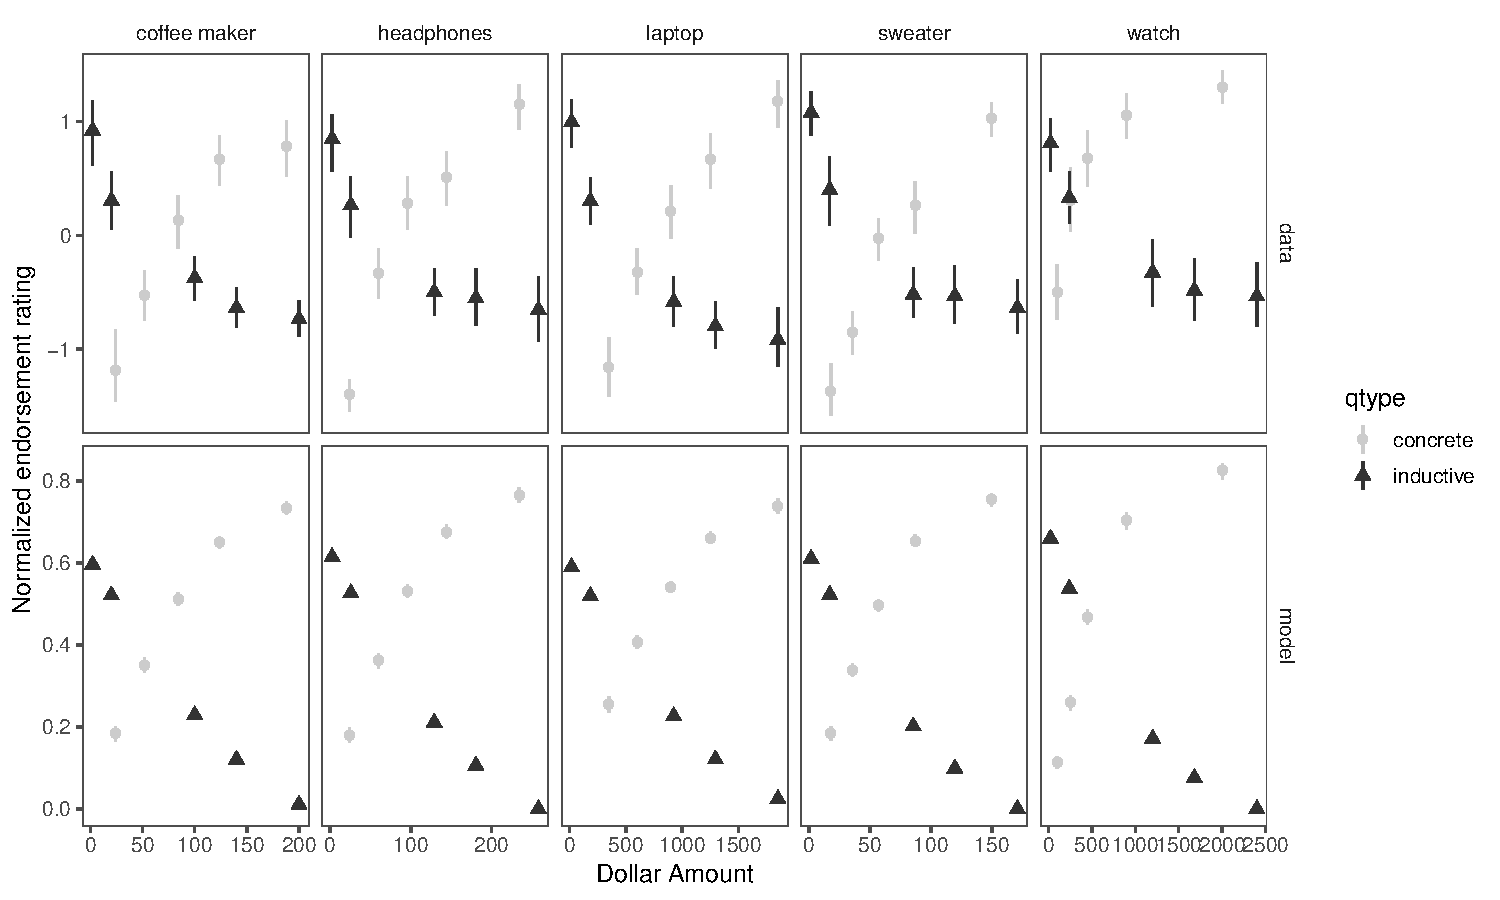
\includegraphics[width=\textwidth]{../analysis/img/reproduce_old_plots_inductive_s1_fit_cost_model.pdf}
\caption{Model fit for final experiments}
\end{figure}

\begin{figure}
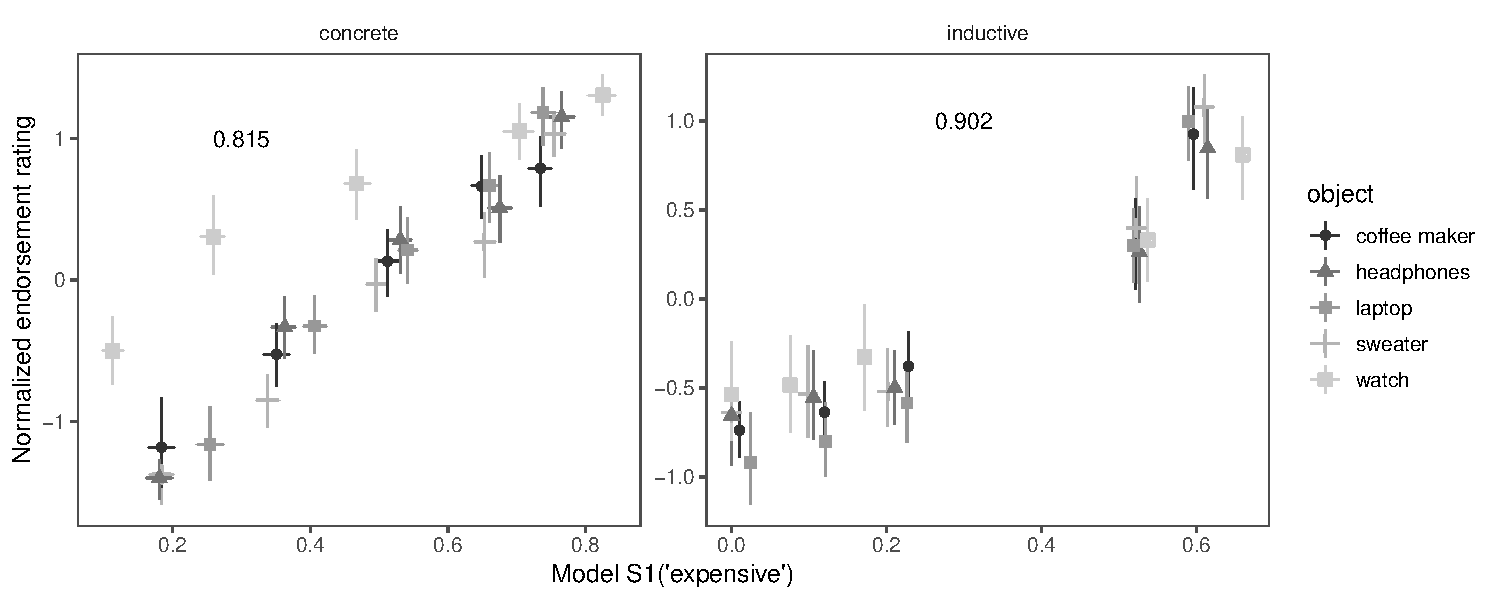
\includegraphics[width=\textwidth]{../analysis/img/reproduce_old_plots_inductive_s1_fit_cost_cor.pdf}
\caption{Final experiments correlations}
\end{figure}

\section{Experiment 3}
\label{exp3}

expt 3a and 3b: getting a wider range of endorsement. 

model fits.

\section{Experiment 4???}

\section{General discussion}
\label{gd}

  -yay. 
  
  -extending to other adjectives and scales?
  
 \subsection{Relation to other theories of vagueness}
  
is this a version of epistemicism? of supervaluation? relation to fuzzy logic?

"Stephen Schiffer (2003, 204) denies that classical probability calculations apply in vague contexts. Suppose Ned is borderline old and borderline bald. According to Schiffer we should be just as confident in the conjunction ?Ned is old and bald? as in either conjunct. [...] He crafts the rules for vague partial belief to provide a psychological solution to the sorites paradox." (SEP)
  
 maybe un-lifted threshold model is a version of epistemicism (there is a threshold, each listener is uncertain what it is).
 
supervaluation seems to be related to disambiguating by choosing a meaning at the literal level that is applied to all instances of a word? but however it works it doesn't seem to account for graded endorsement -- just rejection of truthity.

contextualism: "Scott Soames (2002, 445) answers that all vague words literally are indexical." (SEP)
"Hans Kamp, the founder of contextualism, maintained that the extension of vague words orbits the speaker's store of conversational commitments. In a more psychological vein, Diana Raffman says changes in context trigger gestalt shifts between look-alike categories." (SEP)
"Stewart Shapiro integrates Kamp's ideas with Friedrich Waismann's concept of open texture. Shapiro thinks speakers have discretion over borderline cases because they are judgment dependent." (SEP)

It's worth reflecting on Kamp and Partee's "Prototype theory and compositionality" (Cognition, 1995). (http://semantics.uchicago.edu/kennedy/classes/s06/readings/kamp-partee95.pdf)
  
\subsection{Other vague language}

vague nouns. 

higher-order vagueness.

\section{Conclusion}




\end{document}
